This layer is going to be the interaction layer between the users and the instrument. It consists of a frame possibly made from wood or 3D printed plastic parts. Lasers and photo-resistors will be lodged in to the cavities of the frame. A mister will be there to increase visibility. Traditional 5mm RGB tri-color LED will act as indicators for which lasers were interrupted. Amazon-Basics speakers with frequency range from 103 Hz - 20 KHz will be used for the output sound.

\subsection{Layer Hardware}
This layer will consist of traditional speakers,USB connected misters, LEDs,laser diodes and photo-resistors.

\subsection{Layer Operating System}
Teensy 3.6 will detect the any breakage in the circuit which will be encoded as MIDI signals.

\subsection{Layer Software Dependencies}
Basic C++ arduino script will be running on the teensy to detect any circuit changes.

\subsection{Lasers and receptors}
This consists of laser diodes and photo-resistors connected to a breadboard which is in turn connected to teensy micro controller which detects the lasers' interruption.

\begin{figure}[h!]
	\centering
 	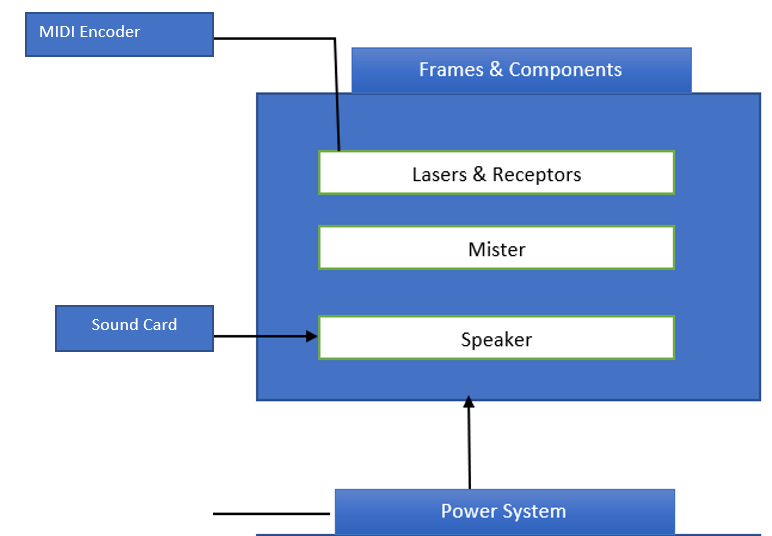
\includegraphics[width=0.60\textwidth]{images/Frame.png}
 \caption{Lasers & Receptors subsystem description diagram}
\end{figure}

\subsubsection{Subsystem Hardware}
Laser diodes will be 6mm 5mW red dot laser head producing 650 nm laser waves running on 5V power supply whereas the photo-resistors are 5 mm GM5539 resistors with spectral peak of 540 nm.

\subsubsection{Subsystem Operating System}
N/A

\subsection{Mister}
It consists of an AGPtck aluminium mini mist maker which will be submerged in water to produce mists which will act as reflective medium for lasers to increase the visibility.

\begin{figure}[h!]
	\centering
 	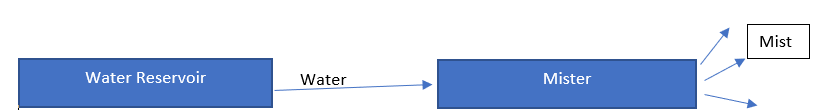
\includegraphics[width=0.60\textwidth]{images/Mister.png}
 \caption{Mister subsystem description diagram}
\end{figure}

\subsubsection{Subsystem Hardware}
A homemade fog machine or a AGPtek mist maker of 1.8 inch diameter with DC 24V power source.

\subsection{Speakers}
They will act as the output of the whole instrument which consists of USB powered speakers for portability.

\begin{figure}[h!]
	\centering
 	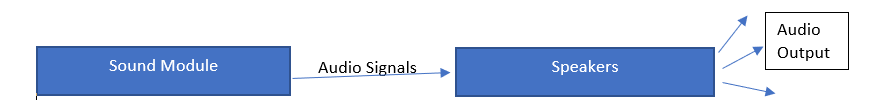
\includegraphics[width=0.60\textwidth]{images/Speaker.png}
 \caption{Speakers subsystem description diagram}
\end{figure}

\subsubsection{Subsystem Hardware}
USB powered speaker(5V) with simple setup having easy front-access control for power and volume.









